\section{Visualising the demographic spatio-temporal evolution}
\label{sec:method}
Figure~\ref{fig:overview} presents an overview of the processing steps of the
proposed method, illustrating how the nodes of the network are used to represent
the regions. The following sections elaborate on this figure and explain the
main features of the interface we built to visualise and explore the evolution
of neighbourhoods on the basis of our proposed method.


\begin{figure}
    \centering 
    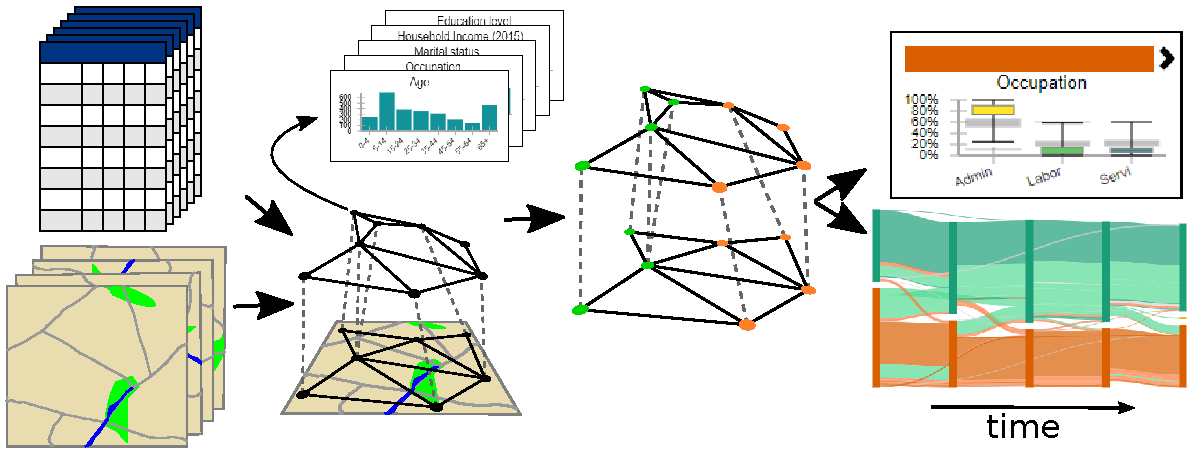
\includegraphics[width=0.975\linewidth]{overview.pdf}
    \caption{Overview of the proposed method. 
        \textbf{(a)} A network is generated from the original data,
        encoding the changing geographical information. 
        \textbf{(b)} The network is partitioned into an hierarchy. 
        \textbf{(c)} The characteristics and evolution of the clusters are then
        visually represented.
        \label{fig:overview}}
\end{figure}


\subsection{Census methodology and data representation}

Census data is disseminated in a tabulated form for aggregation areas: whole
country, state/province, metropolitan region, and so on. To allow for a more
meaningful comparison of the data, we aggregated related variables (e.g. White,
Black, Asian, Other) into what we called an \emph{aspect} (e.g. Race). The
aspects are represented using normalised histograms. This normalisation is
crucial for direct comparison. In essence, it is a generalisation of the
standard method of comparing percentages, since each aggregation area has a
different total population.

Each area of each census year is represented as a node, and edges are placed
between nodes if the corresponding regions share geographic borders in the same
year. Further, edges are placed between nodes if the corresponding regions
belong to sequential years and \revision{1.6/2.6.3}{their geometries intersect.
To avoid spurious connections caused by small fluctuations, one of the
geometries is slightly shrunk before the intersection, using a buffer of -1e6.
While the result would not change considerably by adding more connections
between nearby regions, these extra connections would greatly increase the
computational cost. More importantly, while weights will be associated with
these edges before they are processed, they are not derived from the geometry,
but from the data. The actual intersection area is not considered in this
representation. } This approach leads to a single network representing the whole
spatio-temporal space of the data. 


\subsection{Geographic content clustering}
Having tied the regions together into a network, we can now partition it to
identify similar sets of regions. \revision{2.3}{In essence, we are performing
temporal regionalisation by applying a clustering method over this
spatio-temporal network.}

We start by adopting a distance function between the nodes, measuring the
difference between the data of the regions. This value is then associated with
the edges, leading to a weighted dynamic network. Every node has a collection of
histograms, each representing the distribution of certain aspect in the
population.

Let $\G=(\V,\E)$ be a network, where
$\V=\{\vertice_1,\vertice_2,\dots,\vertice_n\}$ is the set of nodes and
$\E=\{(\vertice_i,\vertice_j), i\not=j\text{ and }i,j \in [1,n]\}$ is the set of
edges. A function $\Hist$ associates each node to a set of $K$ histograms. We
define the distance $\D$ between two nodes $\vertice_i$ and $\vertice_j$ as:

\begin{equation}
    \D(\vertice_i,\vertice_j)=\sum_{k \in [1,K]}{\weight_k\, d(\Hist_k(\vertice_i),\Hist_k(\vertice_j))}
    \label{eq:dist}
\end{equation}

\noindent where $d$ is a distance metric between histograms and $\weight$ is a
sequence of non-negative weights associated with each aspect,
$\sum_{k\in[1,K]}{\weight_k}=1$. While any histogram metric can be used, we
adopted a euclidean distance between the vectors, because it led to reasonable
results with reduced computational cost. Therefore the distance between two
nodes is defined as the weighted average distance between its associated
histograms, where the weights can be adjusted by the user.

Once the distances are associated to the edges, we use watershed
cuts~\citep{Cousty2009} to create an initial clustering, which is then refined
into a hierarchy using the Sorted Maximal Matching (SMM)~\citep{markus2017}. The
initial watershed step is performed to create an initial clustering and reduce
the running time of the SMM. We introduced one new parameter to this method: a
maximum distance threshold for the merges, to avoid the early merging of
outliers. We refer the reader to the original paper~\citep{markus2017} for more
details, including a complete performance evaluation using several metrics.
\revision{1.5/2.2}{We chose this algorithm because it is fast,
simple, and easily customisable, but our methodology should work with any
hierarchical network clustering algorithm. However, we caution against the use
of single-linkage methods due to their tendency to form chain-like clusters with
elements that are similar pairwise, but significantly different on the ends.
That is also the reason we did not use a Watershed hierarchy
directly~\citep{najman2011equivalence}.}


Each resulting cluster is contiguous in the network. This means that two
similar, but non-contiguous, sets of areas will be classified into two different
clusters, which can be counter-intuitive. To overcome this issue, we
\emph{augment} the network with two new edges per node from a nearest neighbours
graph~\citep{scikit-learn} using only the distances between the histograms.
These edges connect nodes with similar content, if they are not already
connected, providing a path for the algorithm to group similar nodes.
\revision{2.4}{The regions connected by those edges will be merged on the first
stages of the clustering, since the nodes they connect are, by definition, as
similar as possible\footnote{This assertion relies on the euclidean distance and
its relationship with the space where k-nn operates.}, leaving the remaining
steps of the hierarchy to be determined only by the geographical edges. We
experimented with different numbers of augmentation edges, but the results were
not consistent, since the distribution of the edges is data dependent. Adding
two edges per node was the smallest number of edges that led to stable and
consistent results in the scenarios available in our prototype. Since the
problem of balancing the data space with the geographical space is relevant for
geographical data analysis, this idea potentially warrants further exploration,
beyond the scope of this work.}


\subsection{Cluster characterisation and variable relevance}
\label{sec:relevance}
A crucial step in understanding neighbourhood change is to characterise the
evolving clusters.  The composition of each cluster is represented here by
simple statistical measures, considering each aspect separately. We compute the
minimum, maximum, median, 25\%, and 75\% quantiles for each variable of each
aspect for all clusters in the hierarchy. While interpreting these values is
more complex than interpreting just the average, they provide far more
information about the underlying distribution.


We also use these statistical measurements to discover what characterises each
cluster, that is, what makes it different from the others.  We define the
\emph{relevance} of a variable of an aspect based on the distance between the
\revision{1.8}{interquartile} ranges (IQR) of the clusters in the same hierarchical level. If
the IQRs overlap for all clusters, that variable is not relevant to the
characterisation of the cluster, but if the IQRs are distant, it means that this
specific range of values is something that only occurs in this cluster.
Examining IQRs therefore provides users a straightforward visual method for
determining what variables most clearly define a given cluster.

To allow for an easier visualisation of these ideas, we represent it using an
\emph{enhanced} version of the traditional boxplot, which includes the IQRs for
the other clusters, in slightly larger and faded black rectangles. We also
colour the current IQR according to its relevance, as illustrated in
Figure~\ref{fig:boxplot}. In this example, this cluster is best defined by the
proportion of the population with four or more years of college. The user can
quickly see that this is relevant because the corresponding IQR is coloured with
the highest relevance present in the legend. It is also clear that, while this
cluster includes CTs that have between 10\% to 90\% of people in this variable,
approximately, half of them have about 60\% of the population with four or more
years of college. Since all the other IQRs are well separated, this is a
defining characteristic of this cluster. Conversely, the proportion of the
population with one to three years of college is not relevant, as indicated by
black fill in the rectangle representing the IQR of this cluster, in overlapping
position with the rectangles of the other clusters.

\subsection{Clusters and trajectories}
While the partition of the data into different clusters helps the user to
understand what groups exist and where they are, we are also interested in the
evolution of these groups. To examine this process of evolution directly, we
introduce the concepts\revision{2.6.4}{ of \emph{temporal paths} and \emph{trajectories}. 

We call a temporal path any sequence of nodes in our representation network such
that the temporal information associated with the nodes only increases. For
instance, in Figure~\ref{fig:intuition}, the sequences ACF, ADF, ADG, and BEH
are temporal paths. With harmonised data, as illustrated by the path BEF, the
time-series of each region would form a temporal path, each node would be
connected only to its older and newer versions, and would belong to only one
temporal path. Since our data is not harmonised, more connections are allowed
and each node can belong to an arbitrary number of paths.

Semantically, this is a generalisation of the idea of geographical time-series,
because each temporal path is one possible option for the data to change over
time. Returning to Figure~\ref{fig:intuition}, the paths ACF, ADF, and ADG all
start on the same homogeneous region, but evolve differently over time. In other
words, this network encodes the information that portions of the region A
changed to form regions C and D, but we do not know specifically which parts.
Nor do we need to, since the same region can belong to several temporal paths.
Interestingly, when interpreted in this framework, geographical harmonisation is
a method to split and/or merge nodes so each belongs to a single temporal path.

Since each node in the sequence that forms the temporal paths has an associated
cluster, we can classify the paths based on the sequence of clusters. We call
each unique sequence of clusters present in this result a \emph{trajectory}.
Regions on the same trajectory had the same sequence of clusters, therefore had
similar temporal evolution.}

\subsection{Overview of the prototype interface}
\label{sec:ui}
To validate and explore the results of our methodology, we built a user
interface, illustrated in Figure~\ref{fig:ui}, considering census tract (CT)
level data from the Chicago region between 1970 and 2010. This region is known
for its entrenched racial divide and the emergence of a \emph{'young urban'}
population with a higher education level~\citep{Delmelle2016,Delmelle2017}. More
details are presented in Section~\ref{sec:study}.


\begin{figure*}
    \centering 
    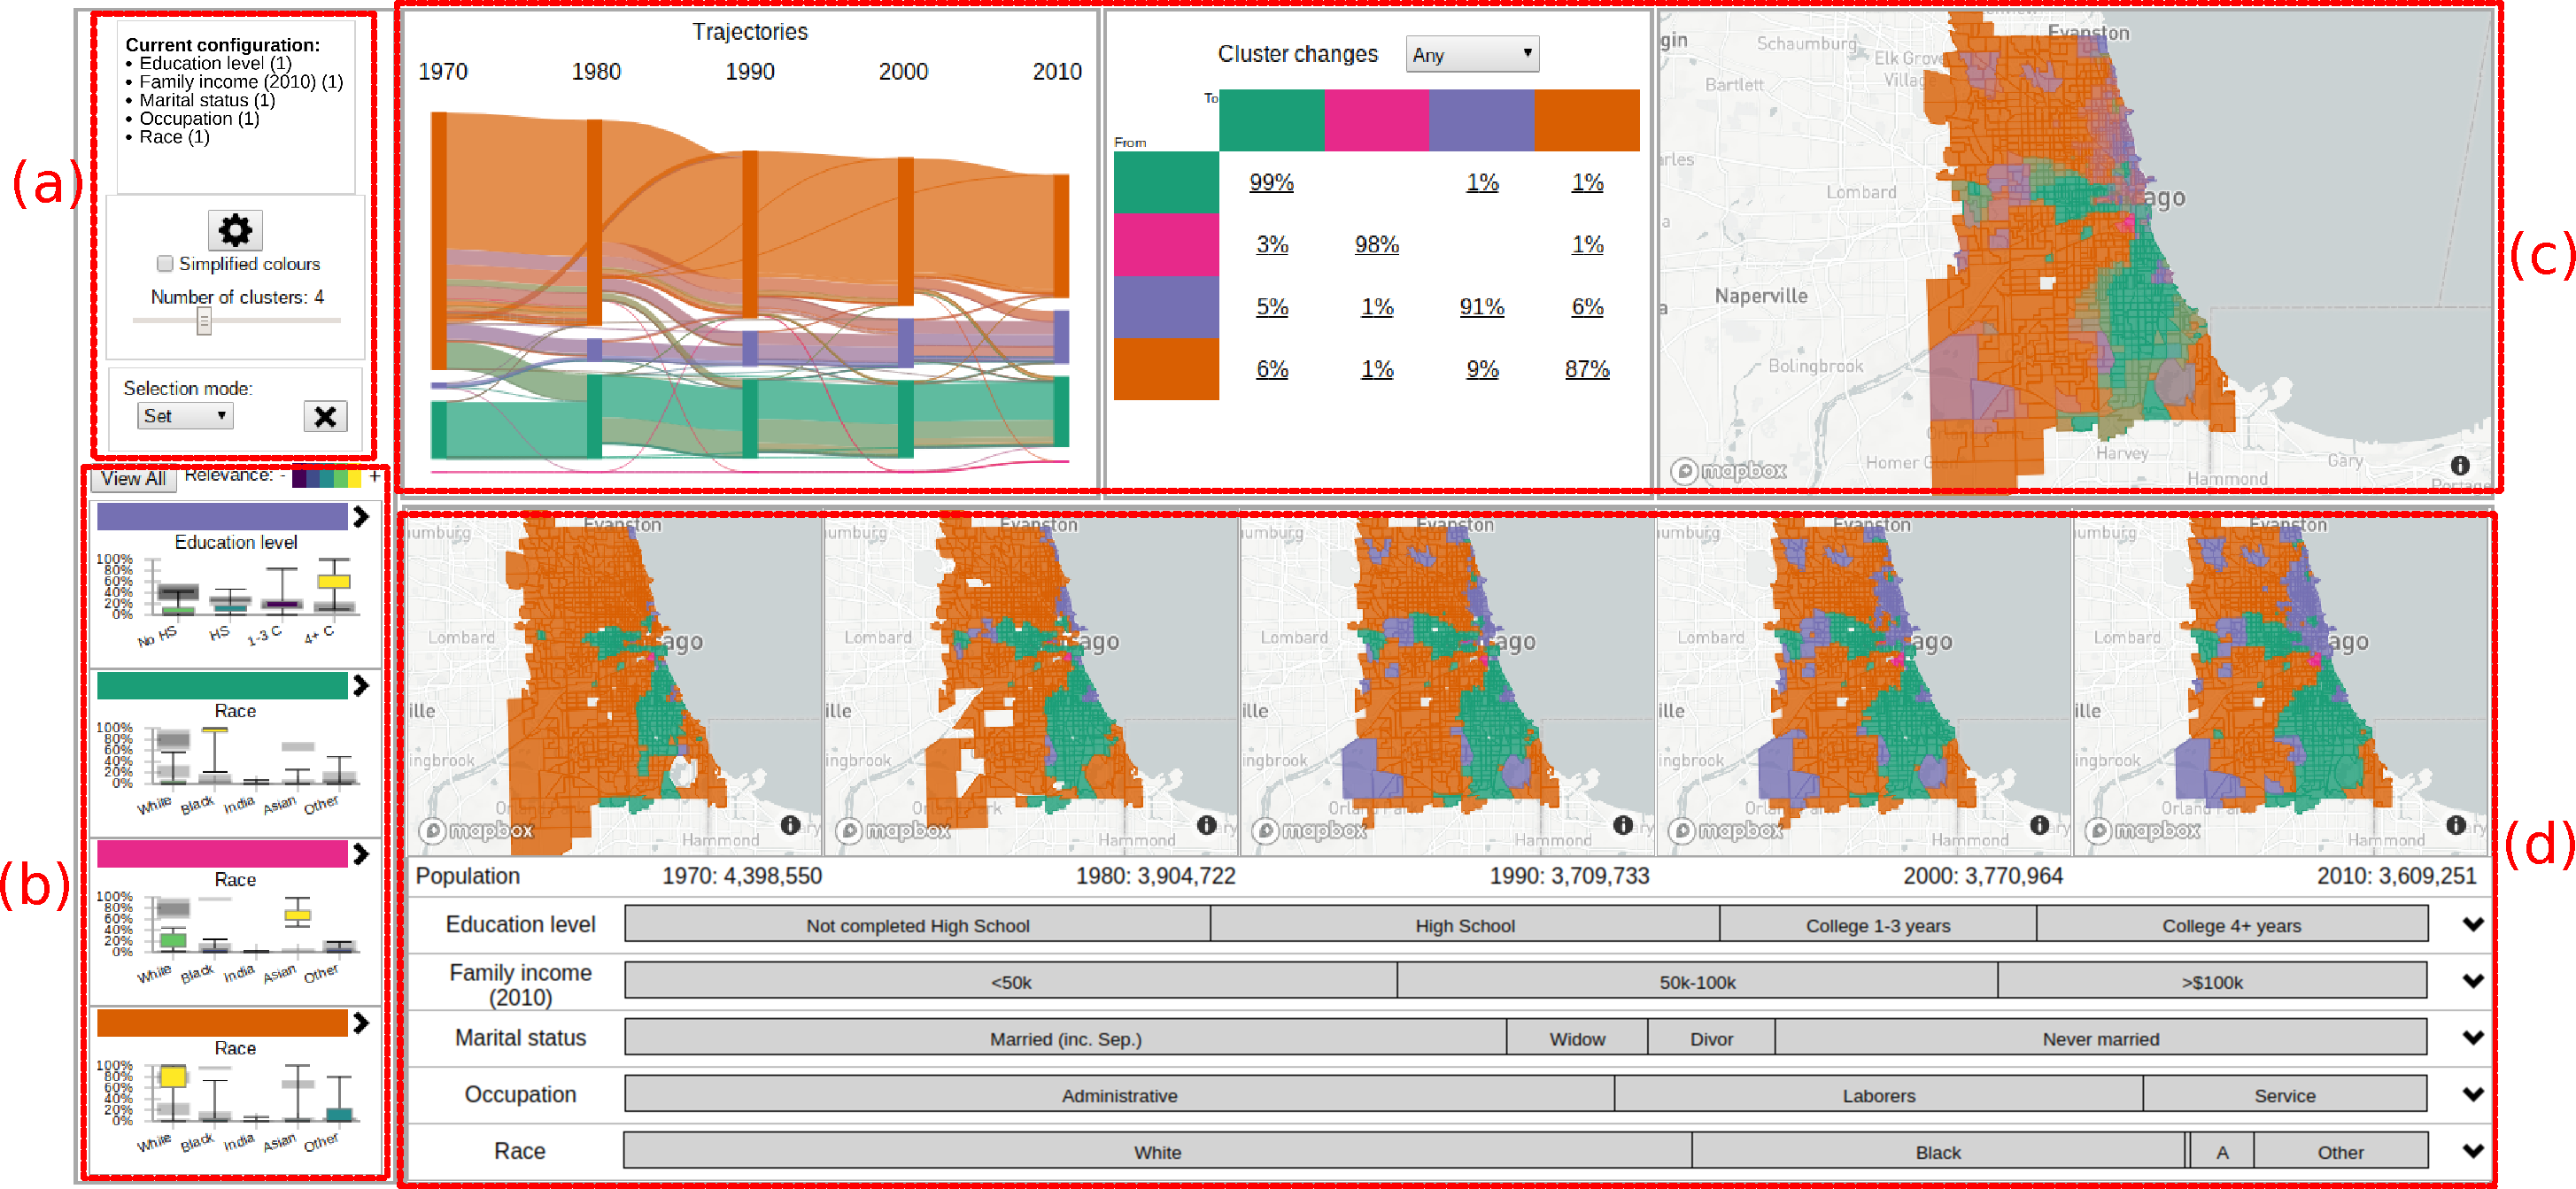
\includegraphics[width=0.975\linewidth]{ui.pdf}
    \caption{Initial interface of our method showing the demographic evolution of Chicago and identifying the objectives of each plot.
        \textbf{(what)}: Cluster overview illustrating the most relevant aspect for each cluster. 
        \textbf{(where)}: Maps illustrating the geographical location, both as an overall summary and for each year.
        \textbf{(how)}: Tabular and visual summmarisation of how the regions classification changed over time.
        \textbf{(who)}: Demographic details for the currently selected data.
        \label{fig:ui}}
\end{figure*}


As illustrated by Figure~\ref{fig:ui}\unsure{CHECK image/ sec 4.5}, our proposed
interface heavily relies on colour to express cluster-related information. We
adopted this convention because colours can be used in all our visual tools in a
coherent manner. However, there is a limit on the number of distinct colours
that can be used. We limited the number of clusters to eight because this was
the largest number of colours that we could reliably and accessibly use, derived
from the 8-class Dark2 set from ColorBrewer~\citep{ColorBrewer}. 


The configuration panel, on top left in Figure~\ref{fig:ui}, displays the
processing configuration of the visualised results: which aspects were used and
their weights (following Equation~\ref{eq:dist}). It also includes other
configuration options that can be altered without re-processing the data, such
as the number of clusters and the colour option. The gear button allows access
to the other configuration options that do require further processing, such as
changing location, aspects, and weights. 

The main functionalities of the interface allow users to examine four
inter-related questions central to understanding local area dynamics. 1)
\emph{What} do the clusters consist in?; 2) \emph{Where} are they located; 3)
\emph{How} do they change?; and 4) \emph{Who} occupy them? We discuss each in
turn.  

The cluster overview panel, marked as \emph{what} in Figure~\ref{fig:ui},
displays the most relevant aspects for each cluster, based on the distance
between the IQRs, as detailed in Section~\ref{sec:relevance}.\revision{2.5}{This
feature allows the user to quickly understand what exists in this region and
which aspect makes each cluster unique, without going into excessive detail. In
Chicago's example, we expect race to be relevant in general, and indeed, it is
recognised as the most relevant aspect for three of the four most distinct
clusters, with the fourth being education level. As we increase the number of
clusters, they get more nuanced, requiring more than one aspect for their proper
characterisation, as each cluster is divided into its composing sub-clusters.
The \emph{View all} button opens a new panel where all aspects are included,
while the chevron at the side lets the user expand each cluster separately,
allowing the exploration of more details on demand.}


\begin{figure}
    \centering 
    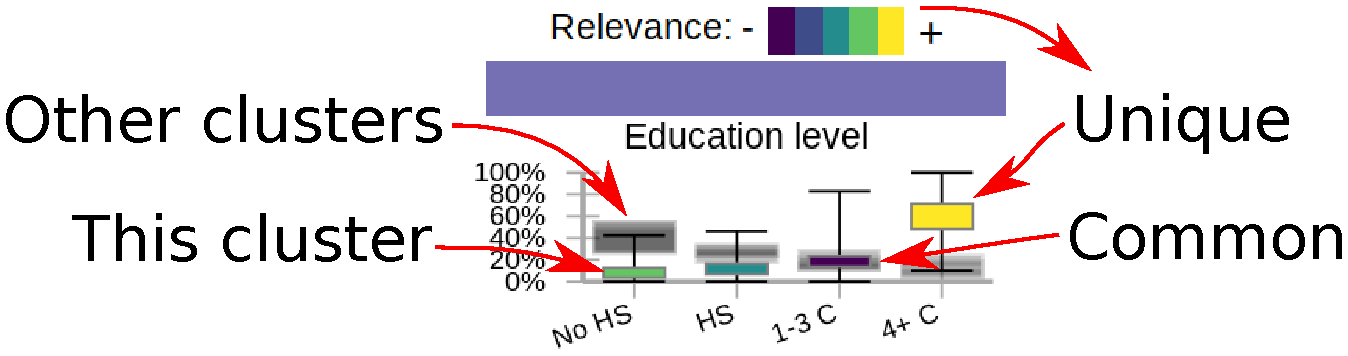
\includegraphics[width=0.45\linewidth]{boxplot.pdf}
    \caption{Enhanced boxplot of the clusters' characteristics allows a quick
    comparison to the other clusters.\label{fig:boxplot}}
\end{figure}


With the knowledge of what clusters are present, we can explore where they are
through the maps, marked as \emph{where} in Figure~\ref{fig:ui}. While the maps
on the lower part of the interface show the location of the clusters at each
time, the larger map shows a summarised version, based on the trajectories of
each region. \revision{1.9}{In simplified mode the colour corresponds to the
cluster present in that trajectory for more than half the temporal samples, and
is grey otherwise. With simplified colours disabled, the colours are the average
of the colours of the clusters in that trajectory in RGB colour
space~\footnote{\url{https://gka.github.io/chroma.js/\#chroma-average}}.}

\revision{2.5}{Each trajectory represents a different temporal path through the
clusters. Therefore the trajectories encode how the demographic characteristics
changed over time. These changes are summarised by the two sections identified
as \emph{how} in Figure~\ref{fig:ui}. In the left panel, there is a Sankey
diagram where each ribbon represents a different trajectory. The widths are
proportional to the population involved.} In our example in Figure~\ref{fig:ui},
the orange and green clusters contain most of the population and are fairly
stable over time. The pink cluster is small and mostly stable. The purple
cluster is increasing, mostly by incorporating areas that were previously
orange. Since the purple group corresponds to the emergent 'young urban' group,
this corroborates the findings of Delmelle~\citep{Delmelle2016,Delmelle2017},
showing that our network-based method can recover results from the traditional
data processing approach.

\revision{2.5}{In the next panel, illustrated in the top middle of
Figure~\ref{fig:ui}, is a transition matrix between the clusters. It indicates a
rounded percentage of regions whose area changed between each pair of
clusters. In this example, we can see that all clusters are fairly stable, with
more than ninety percent of identity transitions.} This kind of table can be
found in the related literature~\citep{Delmelle2016}, so it is familiar to the
advanced users. It not only informs the proportional changes, but allows the
selection of specific changes for further analysis.


The bottom part of the interface contains the details for the selected
trajectories, or for the whole city if nothing is selected, marked as \emph{who}
in Figure~\ref{fig:ui}. The stacked bar plots summarise the overall demographic
composition of these regions. In this example, the maps show the transition from
orange to green and purple in several regions over time. Each aspect is
represented by a stacked bar plot, where the width of each rectangle corresponds
to \revision{1.10}{the percentage of population in that variable over the
considered period. In this case, a little less than half of the population are
married, and the percentage that are Widowers or Divorced is roughly similar.
About half of the population work in Administrative jobs, a third never
completed high-school, approximately forty percent have gross family income
below 50,000USD per year. About sixty percent identify as white. Placing the
mouse over one of the bars will open a small panel with the temporal evolution
of the population percentage of that specific variable, and clicking on the
chevron on the right side expands the corresponding aspect, showing census tract
level statistics, with details of the temporal evolution of each variable and
also the corresponding IQRs for the whole city. Those values differ from the
total population percentage. While the overall population of this region is
about sixty percent White, the average percentage of White population over the
CTs is a little over forty percent.}

More importantly, this interface is fully interactive, allowing for a
progressive exploration of the data. Clicking on a cluster in the cluster
overview panel and the other panels will filter the results to consider only
that cluster, highlighting the geographic regions and involved changes, and
updating population count and demographic composition. If the user selects a
region from the larger map, all identical trajectories are considered, and the
whole interface changes to allow for further study of that specific region.
Clicking on a region in small maps will bring up a new panel with the original
census data of this specific region. Further, these selectors can be combined in
different ways, enabling complex queries with instantaneous results.